\section{Cipher Specifications}
\begin{frame}{Key-Scheduling}
    \begin{block}{}
        Master Key $K$ of 128-bit is divided into two nibbles $k||k'$ each of 64-bit\\
        $k$ - Pre- and Post-whitening\\
        $k'$ - Key-scheduling for the round implementation
    \end{block}
    \begin{block}{}
        $$ k' = k'_{1}||k'_{2}||k'_{3}||k'_{4}||k'_{5}||k'_{6}||k'_{7}||k'_{8} $$
        These 8-bit words are used in key-schedule for generation of the Sub-keys $ f_r(k') $ of different rounds as:
		$$ f_r(k') = k'_{1}||g_r^{(1)}(k'_{2})||k'_{3}||g_r^{(2)}(k'_{4})||k'_{5}||g_r^{(3)}(k'_{6})||k'_{7}||g_r^{(4)}(k'_{8})
		 $$
		where $ 1 \le r \le 20 $ and $ g $ function.
    \end{block}
\end{frame}

\begin{frame}{$g$ function in Key-Scheduling}
    \begin{block}{}
        \begin{table}[H]
			\centering
			\begin{tabular}{|c|l|}
				\hline
				$ g_r^{(1)}(x) $ &  $ (x + 193r) \% $ 256 \\ \hline
				$ g_r^{(2)}(x) $ &  $ (x + 165r) \% $ 256 \\ \hline
				$ g_r^{(3)}(x) $ &  $ (x + 81r) \% $ 256 \\ \hline
				$ g_r^{(4)}(x) $ &  $ (x + 197r) \% $ 256 \\ \hline
			\end{tabular}
			\caption{$g$ function of PRIDE}
			\label{g}
		\end{table}
    \end{block}
\end{frame}

\begin{frame}{Round Function}
    \begin{figure}
        \centering
        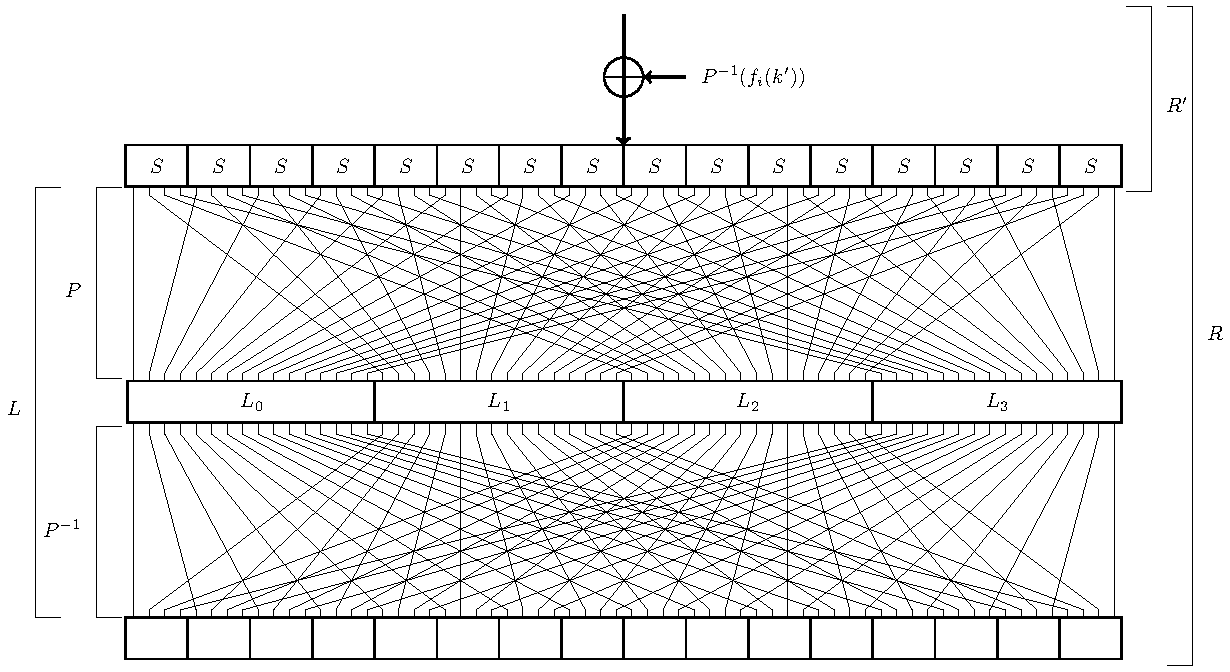
\includegraphics[width=10cm]{pride}
        \caption{Round Function of PRIDE}
        \label{fig:2}
    \end{figure}
\end{frame}

\begin{frame}{Round Information}
    Rounds of PRIDE have different operations as given:
	\begin{itemize}
		\item Round-1 to Round-19 : Key addition, Substitution and Linear Layer
		\item Round-20 : Key addition and Substitution
	\end{itemize}
	\begin{block}{Key-Addition}
	    Xor-ing the round key and the input of the corresponding round.
	\end{block}
\end{frame}

\begin{frame}{Round Information}
    \begin{block}{Substitution layer}
        Output after the key-addition operation is applied into a 4x4 S-Box (i.e to each nibble of the state).
        \begin{table}[H]
		\centering
		\begin{tabular}{c|c|c|c|c|c|c|c|c|c|c|c|c|c|c|c|c}
			\hline
			$x$ & 0 & 1 & 2 & 3 & 4 & 5 & 6 & 7 & 8 & 9 & $ a $ & $ b $ & $ c $ & $ d $ & $ e $ & $ f $ \\ \hline
			$S(x)$ & 0 & 4 & 8 & $ f $ & 1 & 5 & $ e $ & 9 & 2 & 7 & $ a $ & $ c $ & $ b $ & $ d $ & 6 & 3 \\ \hline
		\end{tabular}
		\caption{S-box of Cipher PRIDE}
	\end{table}
    \end{block}
\end{frame}

\begin{frame}{Round Information}
    \begin{block}{Permutation layer}
        This consists of 3 different sub-operations
		\begin{enumerate}
			\item Application of bit permutation $P$.
			\item Application of matrix $ L_i $, for $ i = 0,1,2,3 $ to the $ i^{th} $ word (16-bit) of the state.
			\item Application of bit permutation $ P^{-1} $.
		\end{enumerate}
    \end{block}
\end{frame}

\begin{frame}{LINEAR LAYER}
\begin{block}{LINEAR LAYER OF PRIDE CIPHER}
    \begin{itemize}
            \item Use block interleaving construction
            \item Similar to s-box search of ULLrich et al
            \item search performed on hardware platform instead of software platform
            \item faster search, larger search space
        \end{itemize}
    \end{block}
\end{frame}
\begin{frame}{LINEAR LAYER}
\begin{block}{LINEAR LAYER SEARCH ON HARDWARE}
    \begin{itemize}
            \item Search in a subset of possible 16 * 16 matrices using an FPGA
            \item Limit number of instructions : (CLC,EOR,MOV,MOVW,CLR,SWAP,ASR,ROR,LSL)
           \item Limit number of used regsiters : (2 states,4 temporary registers)
           \item Save the matrices generating appropriate codes
           \item Ended up with 36 instructions for the whole linear layer..
        \end{itemize}
    \end{block}
\end{frame}
\begin{frame}{SECURITY}
\begin{block}{SECURITY}
    \begin{itemize}
           \item Linear and differential cryptanalysis performed
           \item Best possible linear and differential trails generated for 16 rounds.
           \item other attacks(zero-correlation,algebraic)
           \item Further security analysis encouraged..
        \end{itemize}
    \end{block}
\end{frame}